\section{Data collection} \label{sec:rim:dataset}

We collected and constructed three longitudinal datasets to study reviews on Yelp. We present background on Yelp in Section \ref{subsec:rim:background}, we describe the difference between our three datasets in Section \ref{subsec:rim:target_set}, we describe our crawling process in Section \ref{subsec:rim:crawling}, we describe our data organization steps in Section \ref{subsec:rim:organization}, and how to access our data in Section \ref{subsec:rim:availability}.

\subsection{Background} \label{subsec:rim:background}

Yelp breaks reviews into two primary categories, assigned by a software classifer. The categories are ``Recommended'' and ``Not Recommended.'' Yelp lists four reasons for classifying a review as ``Not Recommended:'' conflicts of interest, solicited reviews, reliability, and usefulness. Not Recommended reviews do not affect metrics and are displayed less prominently than Recommended reviews~\cite{yelpwhyrec,yelprecommendationsoftware,yelpstarrating}. In order to study the classifier, it is important that we collect both Recommended and Not Recommended reviews. Yelp also presents a third class for reviews: ``Removed for Violating our Terms of Service,'' which we do not use in our analysis. While Yelp has published an official review dataset for academic purposes~\cite{yelpacademicdataset}, this dataset is not up-to-date and does not include Not Recommended reviews.

We chose to study Yelp because prior work had established reference datasets we could compare against; we chose to use \citet{mukherjee2013yelp}'s dataset of Yelp reviews, collected in 2012, which contains both Recommended and Not Recommended reviews from around 200 restaurants and hotels in Chicago. Furthermore, unlike many other platforms, Yelp allows access to reviews that it does not recommend.

\subsection{Target set selection} \label{subsec:rim:target_set}
Selecting the target set, the set of ZipCodes or businesses to study, required careful selection of sample.


\textbf{Coarse crawl (EYG).} 
The first dataset was a single crawl in which we recrawled the same businesses focused on by \citet{mukherjee2013yelp} Thus, our sample was fixed by the original crawl. Specifically, the Mukherjee et al.~crawl collected all businesses from a target set, then they collected all reviews from the accounts which posted on the targeted businesses, finally they collected metadata for the businesses from those posts. We re-crawled Mukerjee et al.'s target set of businesses, since those are the businesses for which we have the most complete data. We call this the ``eight year gap (EYG)'' crawl because Mukherjee et al.~performed their crawl in 2012 and we performed ours in 2020. By comparing our crawl against Mukherjee et al.'s crawl, we are able to observe reclassifications in the reviews.

\textbf{Fine crawl (CHI).} While our coarse dataset shows changes over a long time scale, it does not reveal how frequently reclassifications occur. To address this, we built a second, finer grained dataset by repeatedly collecting reviews 8 times over 11 months. We chose to use the same ZipCodes so that there would be some intersection with the EYG crawl businesses, ensuring continued crawling of some EYG crawl businesses which helps contextualize those businesses. Because the ZipCodes are within a single metropolitan area, the Chicago area, we call this the ``Chicago (CHI)'' crawl. This more comprehensive but localized coverage of reviews allows for reviewers to be observed posting multiple reviews.

\textbf{Population Density and Income (UDIS / UDS \& UIS).}
Our fine grained dataset gives insight into a local review ecosystem, but it is possible that the sample chosen is not a representative sample. To address this, we collected a third dataset to obtain a broader range of reviews across the US. To allow for the study of reviews in a diverse set of regions, we stratified regions along two axes: one of population density (population per unit area), one of income (median household income). We collected density and income information from the US Census~\cite{acs2019householdincome}, and used ZipCode Tabulated Areas (ZCTAs) as a proxy for ZipCode. ZCTAs approximate USPS ZipCodes, and typically, but not universally, match them~\cite{Census2020zctas}.

For the density stratified crawl, we stratified ZipCodes into 5 strata, dividing the strata evenly by population, using 2019 US Census 5-year American Community Survey data for population estimates~\cite{acs2019populationtotal}. We uniformly sampled ZipCodes from each strata until we had sampled at least 500 businesses from that strata. We included all businesses in each sampled ZipCode, using the Yelp Fusion API to determine the businesses in each ZipCode. We then collected 4 monthly crawls of each dataset. We repeated the same process for the income stratified crawl.

The strata for the income crawls are: \$0--\$55k, \$55k--\$68k, \$68k--\$82k, \$82k--\$105k, \$105k--\$250k. The strata for the density crawls are: 0--67 ppl/$\text{km}^2$, 67--302 ppl$/\text{km}^2$, 302--881 ppl$/\text{km}^2$, 881--1,873 ppl$/\text{km}^2$, 1,873--57,541 ppl$/\text{km}^2$.

Since the union of the income and density data is also a useful dataset as broader sample than the CHI dataset, we present some analyses with individual datasets, ``US Density Stratified (UDS)'' and ``US Income Statified (UIS),'' and some with the combined dataset, ``US Density and Income Stratified (UDIS).''

\subsection{Crawling}\label{subsec:rim:crawling}




\begin{figure}[b!]
    \centering
    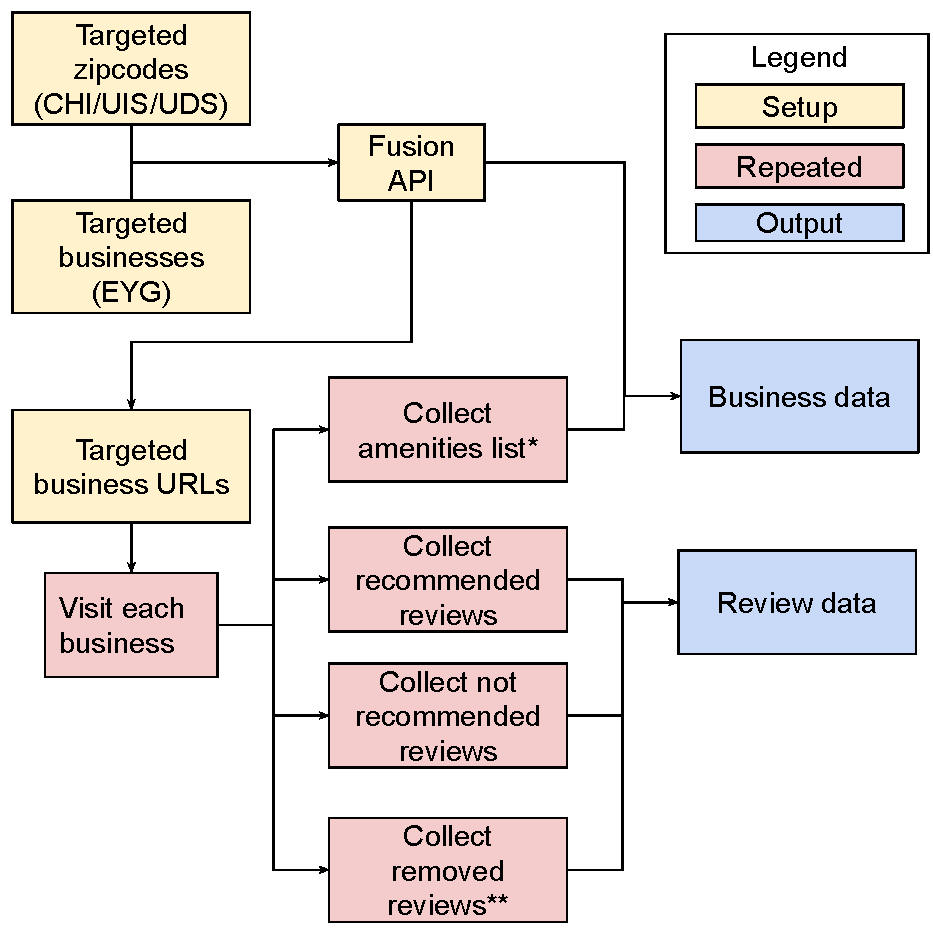
\includegraphics[width=0.9\columnwidth]{chapters/reviews/figures/crawl_diagram.pdf}
    \caption[Data collection process.]{The data collection process. Yellow indicates setup steps that are completed once. Red indicates steps that are completed for each timepoint. Blue indicates outputs.\\
    * We only collected amenities for the CHI 8 and UDIS 4.\\
    ** We only collected Removed reviews for CHI 7-8 and UDIS 3-4. }
    \label{fig:crawling_diagram}
\end{figure}

\begin{table}[t]
    \centering
    \caption{Data and metadata collected.}
    \label{tab:data_collected}
    \resizebox{\columnwidth}{!}{
    \begin{tabular}{l|l}
		  \toprule
            Field & Description \\
			\midrule
			\multicolumn{2}{l}{\textbf{Reviews}}\\
			\midrule
			Content & Text of the review\\
			Author ID & Reviewer identifier (differs for Recommended / Not Recommended reviews)\\
			Date & Date of posting\\
			Rating & Review rating \\
			Business ID & Identifier for the business the review was posted to\\
			Author data & Name and other public account information\\
			Recommended & Whether the review is Recommended\\
			\midrule
			\multicolumn{2}{l}{\textbf{Businesses}}\\
			\midrule
			Business ID & Identifier for the business\\
			Amenities & Listed amenities\\
			\bottomrule
    \end{tabular}
    }
\end{table}

Our crawling occurs in two phases.
First, we have an initial setup phase to collect the set of businesses to crawl. Then we have a crawl phase, where we repeatedly collect reviews. At each crawl timepoint, we visit each of the targeted businesses to collect all reviews on that business. We provide an overview of our crawling process in Figure \ref{fig:crawling_diagram}, and a list of data and metadata collected in Table \ref{tab:data_collected}. 

\textbf{Business data}
To collect our data from Yelp, we first needed to identify the businesses in the target set. For the EYG crawl, we used Yelp's Fusion API~\cite{yelpfusion} to collect business URLs for the business identifiers we had. For the CHI and UDIS crawls, for each targeted ZipCode we used Yelp's Fusion API to collect a list of all businesses. In situations where the search exceeded the API's response limit, we divided our query into multiple queries using other search parameters to reduce the size of the response. We took the union of the businesses returned by all queries and excluded any results that did not have an address with a targeted ZipCodes. For each experiment, once our targeted business list was determined, it remained static for the duration of the experiment.

\textbf{Technologies.}
We used Pyppeteer~\cite{miyakogi2019May}, a Python port of Puppeteer, to build our webcrawler. We ran our crawler in headless mode to reduce system resource utilization. To mitigate IP bans for crawling, we performed our crawl over a VPN.

\textbf{Crawling procedure.}
The crawling process was as follows: we iterated over each ZipCode, then each business (in a non-deterministic order). 
We navigated to the business's page, navigating through the list of Recommended reviews. If we detected any inconsistencies in the page, we retried crawling the business. If we received a block page or exceeded 100 page loads since we changed our VPN connection, we connected to a new VPN server. We then navigated to the Not Recommended reviews, where we repeated the same process to collect Not Recommended and Removed reviews. Yelp added an option to include vaccine and mask requirements in early August, 2021 \cite{yelp2021vaccination}. For crawls beginning after mid-August, 2021, we collected the list of ``amenities,'' which includes mask and vaccine requirements. 

\begin{figure}[h!]
    \centering
    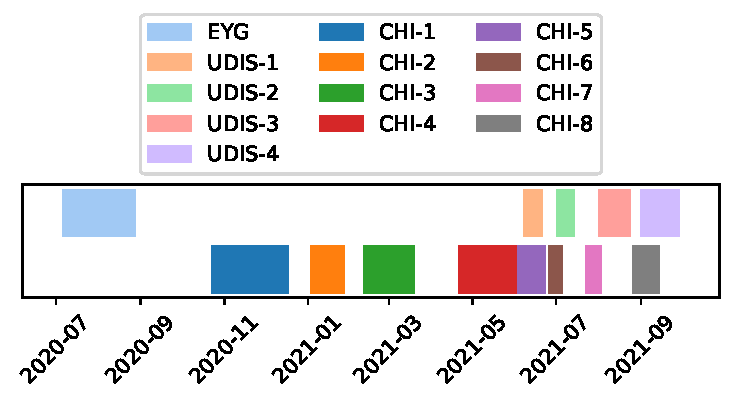
\includegraphics[width=0.9\columnwidth]{chapters/reviews/figures/crawl_timeline.pdf}
    \caption[Crawl timeline]{The timeline for each crawl. Each box indicates the first and last operation for each crawl.}
    \label{fig:crawl_timeline}
\end{figure}

The CHI and UDIS crawls were repeated multiple times to allow for a longitudinal perspective. We refer to crawl time-point by the dataset name and 1-indexed count (e.g. CHI-3 is the third crawl of the CHI dataset). We show the timeline of the crawls in Figure \ref{fig:crawl_timeline}.

\textbf{Quality checks.}
Prior work has shown that web crawls using automation tools and headless browsers are easily detectable, and a website could choose to alter content delivered to automated clients \cite{jueckstock2021towards}. In light of this, we performed two checks to ensure the quality of our data. First, we performed an automated check to measure review attrition and introduction, the percentage of reviews present in crawl $A$ but not in crawl $B$ or vice-versa. Choose two crawls $(A,B)$, where crawl $A$ precedes crawl $B$. Let $R_A$ be the set of reviews for crawl A. For each pair of crawls $\left(A,B\right)$, we checked $\frac{\left|R_A \setminus R_B\right|}{\left|R_A\right|}$ and $\frac{\left|R_B \setminus R_A\right|}{\left|R_B\right|}$. These values never exceed 4.5\% for any pair of adjacent crawls, nor 11\% for any pair of crawls, for either UDIS or CHI. Second, we did a manual check to ensure we collected reviews as they appear for a real user. We randomly selected 50 businesses and a random review position in these business. We manually retrieved the review at that position. Of these reviews, 49 were in our dataset, and 1 was posted after our collection ended.

\textbf{Ethics}
We identify two sources of ethical concerns with our study: the first is the privacy of the user data we have collected, and the second is the impact of our research on Yelp's servers. While all data collected is, or at one point was, publicly available, the review authors did not agree to have their data included in the study. In particular, we treat fields like author name, author location, and review text as sensitive. Therefore, we will require researchers requesting sensitive data to provide an adequate justification for access. To minimize the impact of our research on Yelp's servers, we limited the number of simultaneous crawling threads as much as possible, never exceeding six. We throttled our crawlers to reduce the impact, and we built our crawlers to minimize the pages scraped.

\subsection{Post-processing and organization} \label{subsec:rim:organization}

We took some additional steps to clean up and organize our data.

\textbf{Deduplication.}
Our data has some duplicates. It is possible that some of these are real; for example, if the author accidentally submitted the review twice. However, it is also possible that because our crawls were not instantaneous, review order sometimes shifted during crawling, occasionally leading to double collection of the same review. In either case, such reviews may affect the accuracy of the analysis, and thus we removed these reviews.
To remove duplicate reviews, we removed reviews where all fields (e.g. text, author, date) are identical, retaining one copy.

In our CHI-3 crawl,
approximately 85,000 reviews appeared under both Recommended and Not Recommended, and appeared under Recommended for the adjacent crawls (CHI-2/CHI-4). This coincides with a major update to the Yelp recommendation software~\cite{yelp2021updates}. This event boosts the number of double reclassifications approximately 80-fold if we treat these reviews as Not Recommended, since they are Recommended in CHI-3, Not Recommended in CHI-4, and Recommended in CHI-5. To address this anomaly, we keep the Recommended version of the review and discard the Not Recommended version.

\textbf{Matching reviews.}
We do not have a unique identifier for reviews, so we rely on heuristics to identify instances of the same review across crawls. To determine if two reviews match, we find all reviews with the same text. If two such reviews appear in the same crawl, we discard all reviews with that text, because we cannot disambiguate them (0.04\% of reviews for CHI and 0.04\% for UDIS). Otherwise, we assume the reviews with that text are the same review.

\textbf{Determining authorship.}
Unlike prior work~\cite{mukherjee2013yelp,rayana2015collective}, we were unable to find a universal identifier for authors. Instead, we found two sets of author identifiers: one for Recommended reviews, one for Not Recommended and Removed reviews. This may be due to site design changes on Yelp. We considered matching authors based on metadata but observed too many false positives to consider this approach reliable. However, for authors with at least one reclassified review, the combination of both identifiers serves as a universal identifier. Thus we focus our investigation of authorship on authors with at least one reclassified review.

\textbf{Composition.} After completing the above cleanup and organization steps, we can examine the composition of the datasets. Table \ref{tab:composition} outlines the scale of the datasets after taking the above steps. CHI is the largest dataset in number of timepoints, number of reviews, and number of unique reviews, while EYG has the longest timespan.

\begin{table*}[]
    \centering
    \caption[Dataset composition]{Composition of the datasets. ``\# reviews'' is the number of reviews collected; each review counts each time it is observed. ``\# unique reviews'' is the number of unique review texts. ``\# businesses'' is the number of businesses for which we observed any reviews. The ``\# authors'' range lower bound assumes all unmatched authors of Not Recommended reviews have a Recommended review in the dataset; the upper bound assumes they do not.
    ``\% Recommended'' is averaged across all time-points. EYG data includes reviews from \citet{mukherjee2013yelp}'s crawl.}
    \label{tab:composition}
    \resizebox{\textwidth}{!}{
        \begin{tabular}{lc|c|c|c}
             & EYG & CHI & UDS & UIS \\
    Timespan & 8 years & 11 months & 4 months & 4 months \\
    \# Reviews & 263,308 & 10,485,007 & 1,409,059 & 1,145,995 \\
    \# Unique reviews & 196,383 & 1,395,870 & 358,184 & 292,107\\
    \# Businesses & 201 & 5,773 & 2,829 & 2,843\\
    \# Time-points & 2 & 8 & 4 & 4 \\
    \# Authors (range)  & 100,713 - 119,037 & 404,706 - 520,195 & 212,348 - 259,862 & 180,994 - 221,591\\
    \% Reclassified & 8.69\% & 0.87\% & 0.54\% &  0.61\%\\
    \% Recommended & 88.19\% & 88.90\% & 85.69\% & 85.22\% \\
        \end{tabular}
    }
\end{table*}

\subsection{Availability} \label{subsec:rim:availability}
Our crawling and analysis software is available at \url{https://sites.google.com/princeton.edu/longitudinal-review-data/}. Our dataset is available for researchers to access, with the text of reviews and authors' information replaced by a unique identifier. If the text of reviews or author data is needed, a special request can be made for that information.
